\documentclass[aspectratio=169]{beamer}
\usepackage{color,amsmath}
\usepackage{subfigure}
\usepackage{booktabs}
\usepackage{framed}
\usepackage{comment}

\def\vf{\vfill}

%%%%%%%%%%%%%%%%%%%%%%%%%%
\title[]{Distributed data collection}
\author[]{Matthew J. Salganik\\Department of Sociology\\Princeton University}
\date[]{Summer Institute in Computational Social Science\\June 23, 2018
\vfill
\begin{flushleft}
{\scriptsize
The Summer Institute in Computational Social Science is supported by grants from the Russell Sage Foundation and the Alfred P. Sloan Foundation.}
\end{flushleft}
\begin{flushright}

\includegraphics[width=0.1\textwidth]{figures/cc-by.png}
\end{flushright}
}
\begin{document}
%%%%%%%%%%%%%%%%%%%%%%%%%%
\frame{\titlepage}
%%%%%%%%%%%%%%%%%%%%%%%%%%
\begin{frame}

\begin{itemize}
\item people can be where the researchers can't
\pause
\item scale that researcher cannot match
\pause
\item sometimes hard to separate from human computation
\end{itemize}

\end{frame}
%%%%%%%%%%%%%%%%%%%%%%%%%%
\begin{frame}

\begin{center}

\includegraphics[width=0.6\textwidth]{figures/photocity_logo}
\end{center}

\small{
Tuite et al. (2011) ``PhotoCity: Training Experts at Large-scale Image Acquisition Through a Competitive Game'' \textit{CHI}:  \url{http://dx.doi.org/10.1145/1978942.1979146}
}

\end{frame}
%%%%%%%%%%%%%%%%%%%%
\begin{frame}

\begin{center}
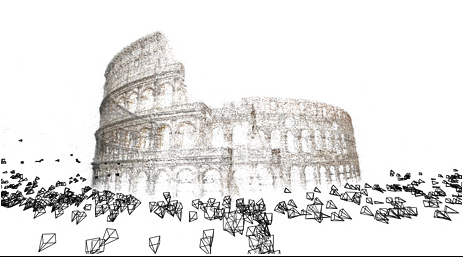
\includegraphics[width=0.6\textwidth]{figures/rome_in_a_day}
\end{center}
Rome in a Day (Agarwal et al., 2009)

\end{frame}
%%%%%%%%%%%%%%%%%
\begin{frame}

\begin{center}
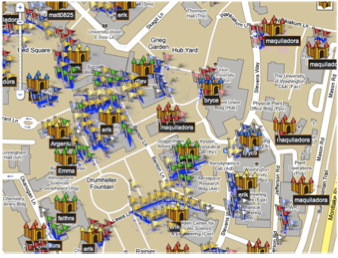
\includegraphics[width=0.6\textwidth]{figures/tuite_photocity_2011_fig2}
\end{center}

Two campuses: University of Washington and Cornell University

\end{frame}
%%%%%%%%%%%%%%%%%
\begin{frame}

Over 2 months, 100,000 photos submitted by 45 players
\vf
\begin{center}
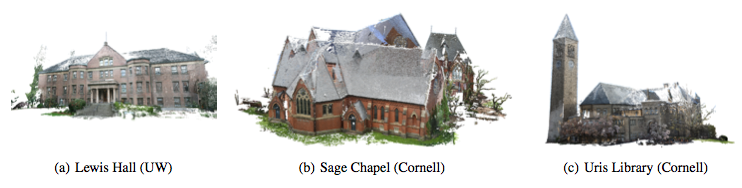
\includegraphics[width=0.9\textwidth]{figures/tuite_photocity_2011_fig8}
\end{center}

\end{frame}
%%%%%%%%%%%%%%%%%
\begin{frame}
\frametitle{PhotoCity}

Beautiful design solves lots of problems
\pause
\begin{itemize}
\item data collection is standardized because of cameras
\pause
\item verification is automatic by comparison with nearby images
\pause
\item game points are assigned based on the value of data, trains people to collect more valuable data
\end{itemize}

\end{frame}
%%%%%%%%%%%%%%%%%%%%%%%%%%
\begin{frame}

{\Large
\begin{center}
Questions?
\end{center}
}

\end{frame}
%%%%%%%%%%%%%%%%%%%%%%%%%%

\end{document}
